\documentclass[12pt]{article}

% Packages
\usepackage{amsmath, amssymb} % math symbols
\usepackage{enumitem}         % better control over lists
\usepackage{hyperref}         % clickable links
\usepackage{graphicx}

% Title Info
\title{ESE5320 Homework 2}
\author{Rico Zhuang}
\date{September 12, 2025}

\begin{document}

\maketitle

\section*{Answers}

\begin{enumerate}
    \item \textbf{Identify}
    \begin{enumerate}[label=\arabic*)]
        \item \textbf{Scale}: this function downscales an image(stored in a 1d array \text{"input"}) by only outputing every two pixel.
        \\\\ \textbf{Filter}: applies a convolution filter to the image; first horizontally, then vertically, using hard-coded coefficients. It takes the input image to produce a smoothed output image.
        \\\\ \textbf{Differentiate}: for each pixel, use the value of its left pixel and its up pixel to calculate an average, and output will be the difference between that pixel's value and the average.
        \\\\ \textbf{Compress}: This compresses the input array using Huffman coding, packing bits into the output array one byte at a time. It returns the total number of bytes written to the output.


    \end{enumerate}

    \item  \textbf{Measure}


        \begin{tabular}{|c|c|c|c|}
        \hline
        Functions & $T_{\text{measured\_avg}}$(ns) & \% of Total Latency & $T_{\text{measured\_avg}}$(cycles) \\
        \hline
        Scale & 2.09032e+07 & 3.64 & 7.10708+e07\\
        \hline
        Filter horizontal & 1.03589e+08 & 14.57 & 3.52202e+08\\
        \hline
        Filter vertical & 1.04882e+08 & 16.39 & 3.56599e+08\\
        \hline
        Differentiate & 2.59741e+07 & 3.64 & 8.83120e+07\\
        \hline
        Compress & 3.22591e+08 & 61.94 & 1.09681e+09\\
        \hline

        \end{tabular}
        \begin{enumerate}[label=\arabic*)]
        \item Done
        \item Done
        \item Done

% 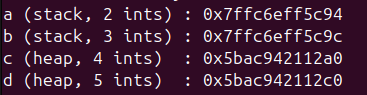
\includegraphics[width=0.6\textwidth]{image5.png}
    \end{enumerate}

    \item \textbf{Analyze}
    \begin{enumerate}[label=\arabic*)]
        \item \begin{tabular}{|c|c|c|}
\hline
Functions & $T_{\text{measured\_avg}}$ (ns) & $T_{\text{measured\_avg}}$ (cycles @ 1.2\,GHz) \\
\hline
Scale             & 8.426840e+08 & 1.011221e+09 \\
\hline
Filter\_horizontal & 5.241310e+09 & 6.289572e+09 \\
\hline
Filter\_vertical   & 5.299610e+09 & 6.359532e+09 \\
\hline
Differentiate      & 1.632450e+09 & 1.958940e+09 \\
\hline
Compress           & 5.363130e+09 & 6.435756e+09 \\
\hline
\end{tabular}
    \item The Scale funtion has the highest latency.
    \item 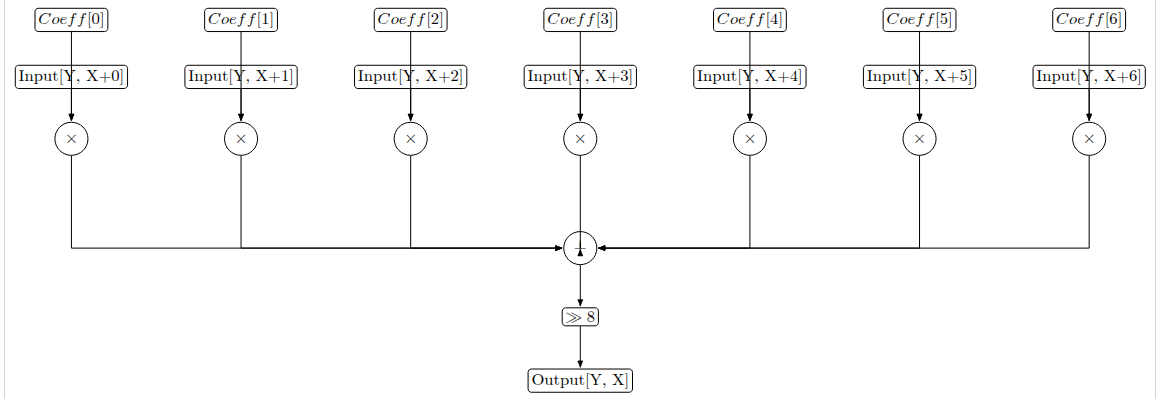
\includegraphics[width=1.0\textwidth]{3_3.png}
    \item total operation count is \textbf{3.35664e+08}, and average latency is \textbf{3.35664e+08} cycles
    \item I would choose \textbf{Compress} because it has the highest latency and therefore will benifit the most from speedups.
    \item function Compress takes about 29\% of total latency, so the maximum possible speedup is 1/(1-0.29) = \textbf{1.4}
    \item todo
    \item critical path length is \textbf{5 operations}
    \item need two cycles for mult, 3 for add and 1 for shift, therefore lower bound is \textbf{3 cycles}

    \end{enumerate}

\end{enumerate}

\end{document}
